\begin{recipe}{烤酥方}

\ingredients

\ingredient{生猪肉}{(约十五斤)一方}
\ingredient{蒜}{四两}
\ingredient{葱}{一斤}
\ingredient{柴}{十斤}
\ingredient{杠炭}{十五斤}
\ingredient{甜酱}{四两}
\ingredient{香油}{一两}

\preparation

\step[选料及处理] 选厚膘连皮带肋骨肉一方,横、长一尺,
\begin{wrapfigure}[9]{l}{15em}%
\begin{center}%
\vspace{-1.5\baselineskip}%
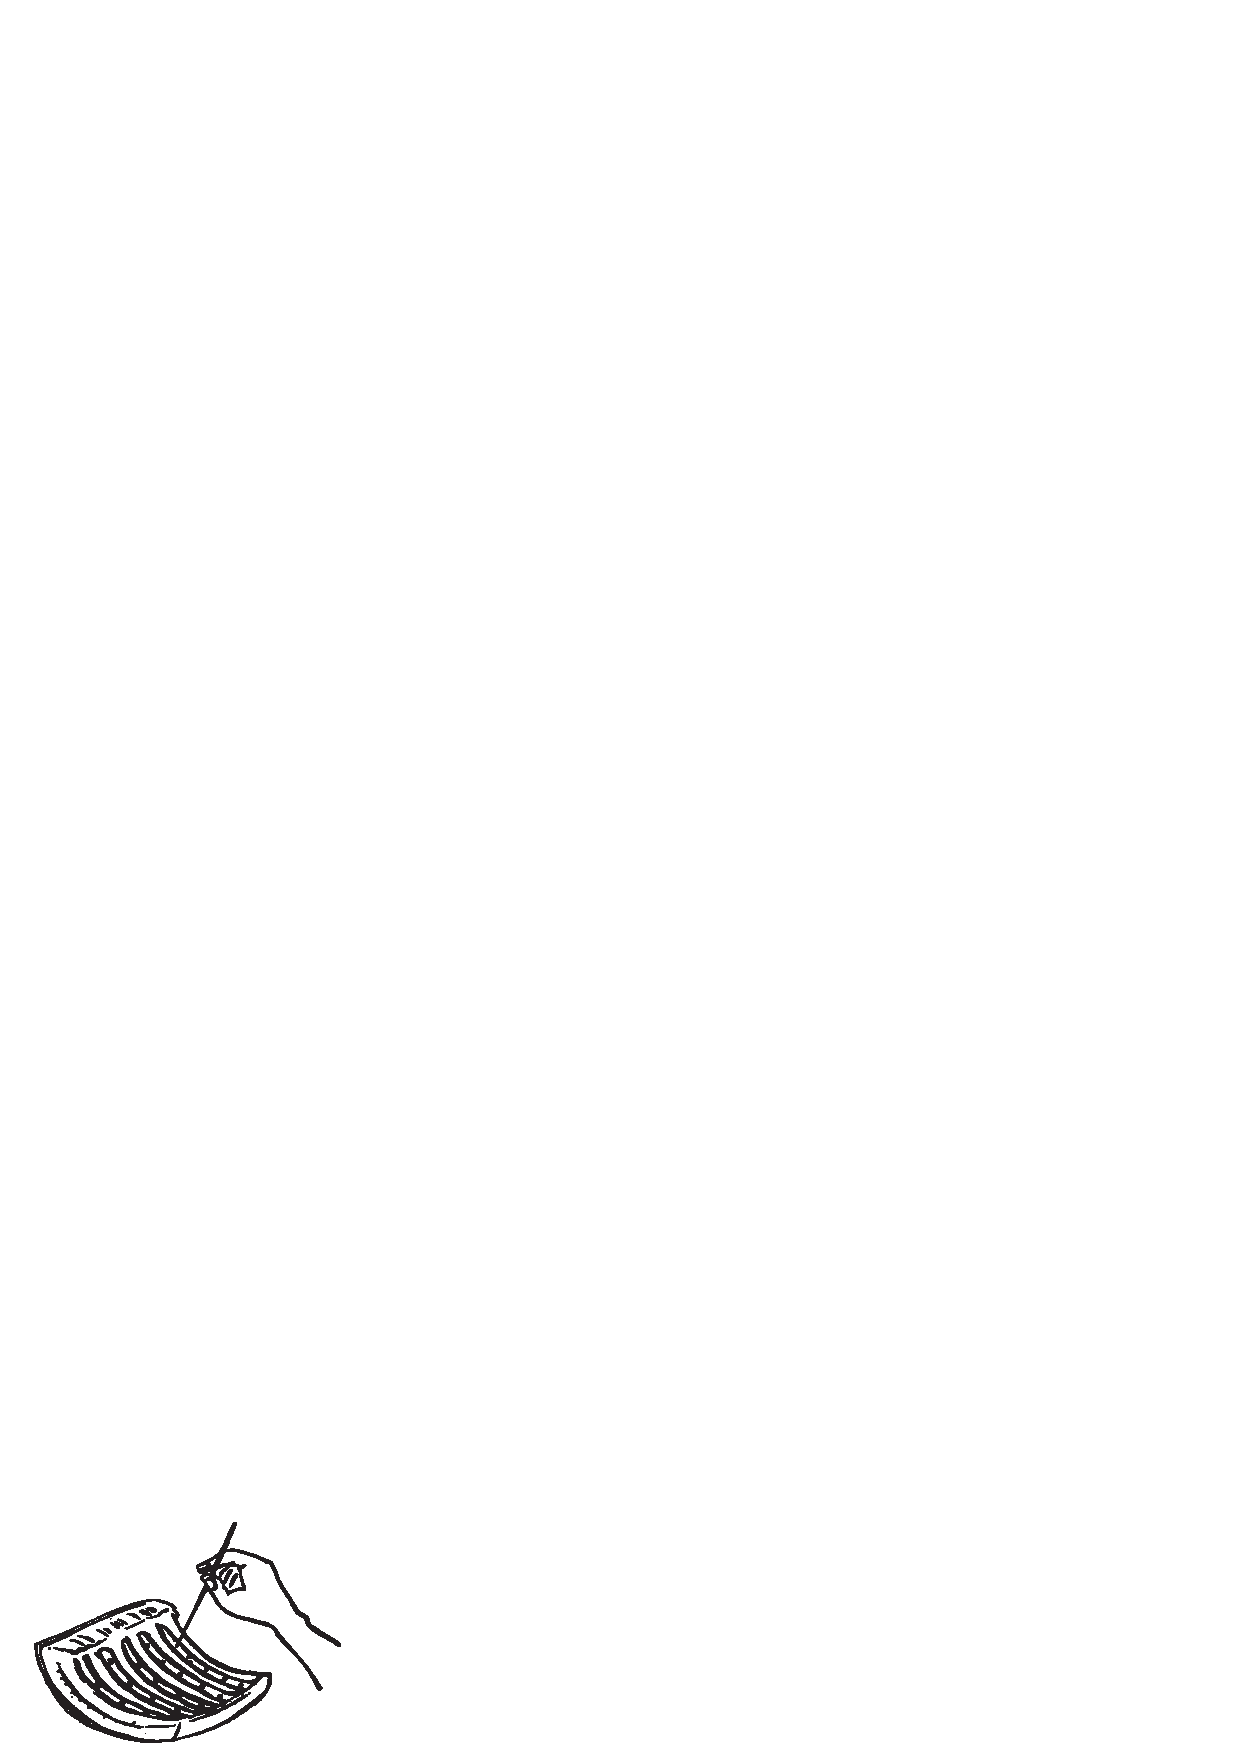
\includegraphics[scale=1]{illustration-005.pdf}%
\vspace{-.1625\baselineskip}%
\caption{刺气眼}
\label{poking holes in the meat}
\end{center}%
\end{wrapfigure}
宽九寸。肉皮须平整没有凸凹者。先去净茸毛,刮洗干净。然后肉皮向下、排骨向上放于
案板上,用直径二分粗的尖长竹签,在排骨缝中瘦肉上刺上若干气眼。刺的深度以接近肉
皮为合适,但不要把肉皮刺破(图~\ref{poking holes in the meat}\,)。然后将它揩
干水份,用铁质二股烤叉一把,由排骨之下,肥肉之上的痩肉中叉进去(图~\ref{forking
the meat}\,),叉尖伸出肉方外约一尺左右。

\begin{wrapfigure}[13]{r}{11em}%
\begin{center}%
\vspace{-2.625\baselineskip}%
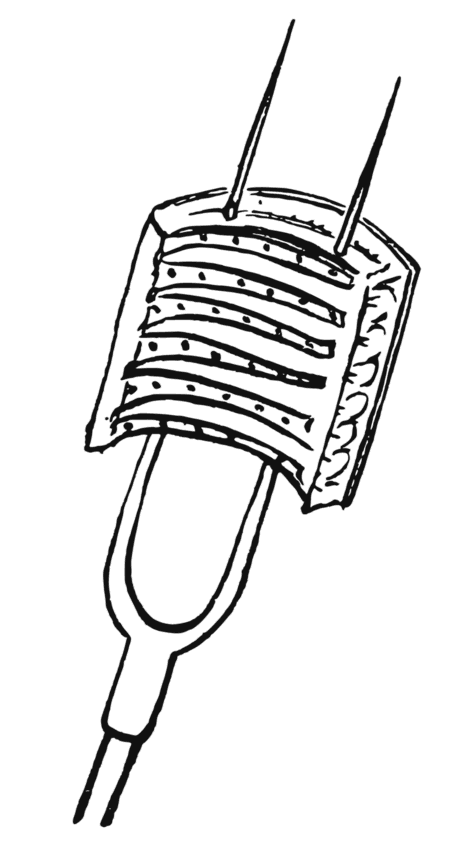
\includegraphics[scale=1]{illustration-006.pdf}%
\vspace{-.625\baselineskip}%
\caption{叉肉}
\label{forking the meat}
\end{center}%
\end{wrapfigure}

\step[出坯] 用干柴十斤,先用二斤放炉内烧燃,炉中火苗燎出炉口一尺至二尺(须经常
保持这种火苗,火苗不均匀时加柴),随即手拿叉柄,将肉方的皮向着火苗,排骨向上
(不要着火)在火苗上燎。一面调剂火候,一面手拿叉柄左右拧动。拧动的角度是:先把
肉方拧至肉皮与地平成八十五度后,再拧过去成同样的角度。这样反复来回拧动。拧动的
速度是:中间稍稍快,两端稍停。着重燎肉方的四周和四角,燎至肉皮上的毛眼中好像在
沸腾。同时猪皮上比较粗老的皮被烤成一层很薄的黑壳,自行整张地脱落于炉火中(若有
的地方没有落,就说明那里的火候还不够),然后将肉方挪开炉火,用净布擦净叉尖,取
下放入烫水中,用布帕洗净。通过出坯,肉皮比原肉皮薄,保留的肉皮约半分厚,皮上微
微现出蜂窝形状的花纹,带牙黄色,本道工序即成。待本菜上席前二十分钟再进行烤酥的
工序。

\step[烤酥] 用青砖二十四块,在平坦的地坪上嵌一烤池,用细煤渣灰五斤平铺在烤池底,
将杠炭八斤烧红,平放(不要
\begin{wrapfigure}[13]{l}{15em}%
\begin{center}%
\vspace{-1.125\baselineskip}%
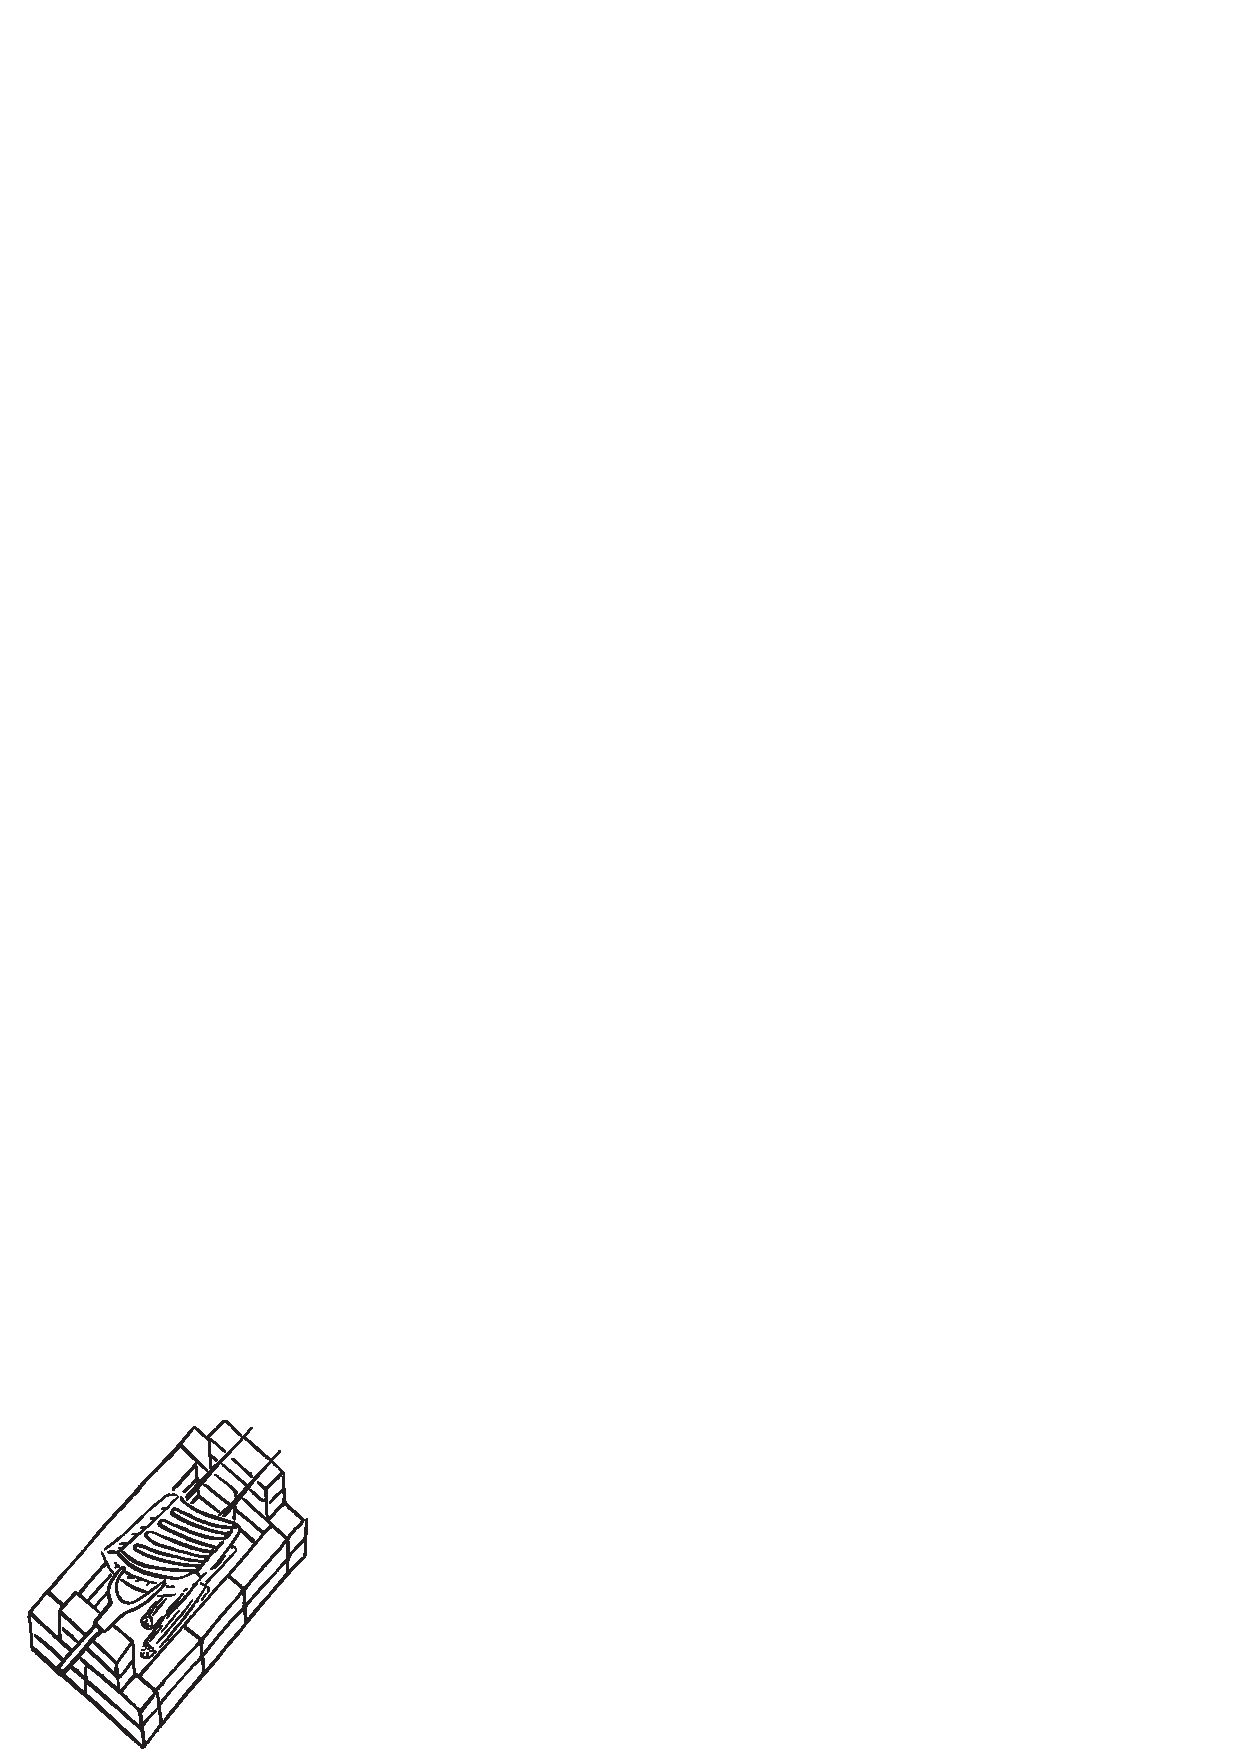
\includegraphics[scale=1]{illustration-007.pdf}%
\vspace{.1875\baselineskip}%
\caption{烤酥}
\label{baking the meat}
\end{center}%
\end{wrapfigure}
立放,立放便要伸出火苗,烤酥时严忌火苗)在烤池之中。再将肉方由原叉眼中叉好,放
于烤池上,肉皮向火,排骨向上(图~\ref{baking the meat}\,),同样手拿叉柄左右拧
动。拧动的角度与出坯相同,但速度稍快。烤至肉方出油时,将烤池内的红杠炭检于烤池
四周(前后两端多放一些,去净池心的火星,以免肉方的油滴于火上,引起火苗),继续
拧动着烤。此时肉方皮上的油很多,为了使它在肉皮上流来流去,把皮烫酥,而不掉下来,
故拧动速度宜再快些。烤至肉皮成金黄色时,可以用刀尖试验一下是否酥泡。试法是:用
手指捏着刀叶,只留一分长的刀尖在外,将肉方拿离烤池,用刀尖在肉皮上连锥几下,如
发出酥泡的响声为合格。然后将香油三钱刷于酥皮之上,用净布擦净叉尖,取下酥方,
酥皮向上放于大圆盘中。

\step[铲皮上席] 用刀尖在酥皮下平铲,将铲下的酥皮切成一寸半长、七分宽的条方片,
照原样摆于肉方之上。另外,给每位顾客配汤盃一个,内盛加味特级清汤\footnotemark
(二两);三寸手碟一个,内盛蒜片、甜酱(甜酱中加香油二钱搅匀)、葱白段(一寸半
长)三段;再配五寸平盘一个,内盛点心两块,连同穌方一同上席。

\step[吃法] 一般只吃酥方皮,不吃肉。肉可用来做回锅肉,别有风味。

\suggestion

烤方需要一定技术,操作中稍不注意,就会发生质量事故。易于发生的质量事故及其补救
方法如下:

\hint[方皮鼓泡] 鼓泡在“出坯”和“烤酥”中都会发生。其原因是气眼刺得不好,或拧动角
度太大。补救方法是:把肉方拿离烤池,用尖头竹签在鼓泡的附近由痩肉中刺眼放气,若
鼓泡太大,可用刀将鼓泡的皮割去,抹上蛋清豆粉,稍抹厚点,再继续烤。

\hint[硬皮] 发生硬皮的原因是“出坯”时火候不匀,或烤酥时拧动角度太小。补救方法是:
将肉方拿离烤池,在池中检红杠炭一块(炭的大小与硬皮相等),逼近硬皮处烤至微焦,
再用小刀将烤焦处之皮刮去一层,继续上烤池烤。

\hint[烂皮] 发生烂皮的原因是出坯时拧动速度太慢,以致肉皮被烧烂。补救方法:用蛋
清豆粉抹烂皮处,厚厚地抹一层,再继续上烤池烤。

\hint[漏油] 在选料或刺气眼没有注意,皮上有眼就会漏油。在烤酥时,可用蛋清团粉抹
严,再继续烤。

\features

此菜一般是高贵筵席的配菜,色彩金黄,美观大方,吃时酥香,脂肪特多,而爽口不腻。

\footnotetext{
\begin{subrecipe}{特级清汤}

\ingredients

\ingredient{老母鸡}{一只(三斤)}
\ingredient{老肥鸭}{一只(三斤)}
\ingredient{火腿蹄子}{一只}
\ingredient{火腿棒子骨}{一斤}
\ingredient{排骨}{二斤}
\ingredient{鸡脯肉}{三个}
\ingredient{猪生瘦肉}{五斤}
\ingredient{清水}{三十斤}

\preparation

\step 将鸡、鸭宰杀,去毛,去内脏。蹄子、棒子骨刮洗干净。生瘦肉、鸡脯肉都分别用
刀背捶成茸。

\step 汤锅放炉上,将棒子骨、排骨、蹄子、鸡、鸭依次放入汤锅中,倒入清水二十五
斤,用旺火烧开,去净泡沫,炖一小时。而后捞出,漂于温热水中。用猪肉茸一斤,加清
水一斤兑匀调散,倒入汤锅中;待瘦肉和泡沫浮起时,用漏瓢打净。将鸡、鸭、蹄、骨等
用热水洗净,放于汤锅中,用微火焅半小时,将鸡、鸭捞出另作别用,再将各骨捞出漂溫
水中。然后将猪肉茸四斤,加清水三斤调散倒于汤锅中;待肉茸浮起时,用漏瓢把它挤成
四至五个肉饼。再将汤面浮油吹净,将各骨用温水洗净,轻轻放入汤锅中;随后将肉饼放
于各骨之上,用小微火焅。此时汤已变色,很象料酒颜色。鸡茸内加清水一斤调散。待使
用清汤时,再将鸡茸倒入汤中,待泡沫和肉茸浮起后,将泡沫和肉茸打去,即成清汤。
\end{subrecipe}
}

\end{recipe}

% vim: filetype=tex noautoindent nojoinspaces
% vim: fileencoding=utf-8 formatoptions+=m
% vim: textwidth=78 tabstop=4 shiftwidth=4 softtabstop=4
